\documentclass[12pt]{article}
\usepackage{light}
\usepackage{enumerate}

\hidesolutions
\showsolutions

\newcommand{\edge}[2]{#1\text{---}#2}
\newcommand{\mfigure}[3]{\bigskip\centerline{\resizebox{#1}{#2}{\includegraphics{#3}}}\bigskip}
\newcommand{\eqdef}{\mathbin{::=}}

\begin{document}

\recitation{6}{September 30, 2016}

%%%%%%%%%%%%%%%%%%%%%%%%%%%%%%%%%%%%%%%%%%%%%%%%%%%%%%%%%%%%%%%%%%%%%%%%%%%%%%%
%\insolutions{
%\stamp
\section*{Graph Basics}

Let $G = (V,E)$ be a graph. Here is a picture of a graph.
\begin{center}
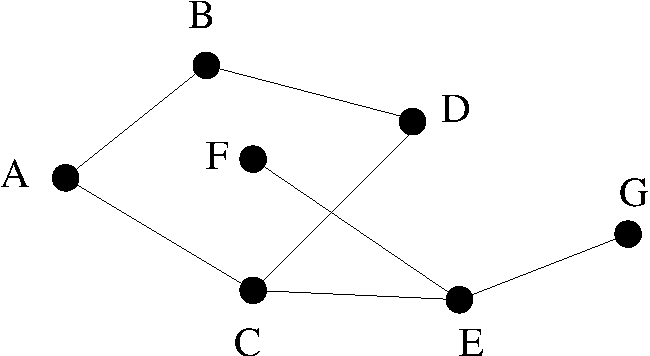
\includegraphics[height=1.75in]{example}
\end{center}
Recall that the elements of $V$ are called vertices, and those of $E$
are called edges. In this example the vertices are $\set{A, B, C, D,
  E, F,G}$ and the edges are $$\set{\edge{A}{B}, \edge{B}{D},
  \edge{C}{D}, \edge{A}{C}, \edge{E}{F}, \edge{C}{E}, \edge{E}{G}}.$$

Deleting some vertices or edges from a graph leaves a {\em subgraph}.
Formally, a subgraph of $G = (V, E)$ is a graph $G' = (V', E')$ where
$V'$ is a nonempty subset of $V$ and $E'$ is a subset of $E$.  Since a
subgraph is itself a graph, the endpoints of every edge in $E'$ must
be vertices in $V'$. For example, $V' = \set{A,B,C,D}$ and $E' =
\set{\edge{A}{B},\edge{B}{D},\edge{C}{D}, \edge{A}{C}}$ forms a
subgraph of $G$.

In the special case where we only remove edges incident to removed
nodes, we say that $G'$ is the {\em subgraph induced on $V'$} if $E' =
\{( \edge{x}{y}| x,y \in V' {\rm ~and~} \edge{x}{y} \in E \}$.  In
other words, we keep all edges unless they are incident to a node not
in $V'$. For instance, for a new set of vertices $V'=\set{A,B,C,D}$,
the induced subgraph $G'$ has the set of edges $E'=
\set{\edge{A}{B},\edge{B}{D},\edge{C}{D}, \edge{A}{C}}$.

Remember in lecture that we covered a graph of actors and actresses. In the graph, there
were two kinds of vertices, male and female, and the edges went only went between both.
This type of graph is known as a {\em bipartite graph}. A graph $G$ = $(V, E)$ is called bipartite if we can divide the vertex set into two parts, the ``left" part and the ``right" part, so that every edge has one endpoint in the left part, and
one endpoint in the right part. The figure below shows an example of a bipartite graph. A {\em matching} means that there is a way of assigning every vertex in the ``left" part to a vertex in the ``right" part so that different vertices in the ``left" part are assigned to different vertices in the ``right" part and there is an edge between assigned vertices. In the graph from lecture, a matching will mean a way of assigning every man to a woman so that different men are assigned to different women, and a man is always assigned to a woman that he likes.
\begin{center}
    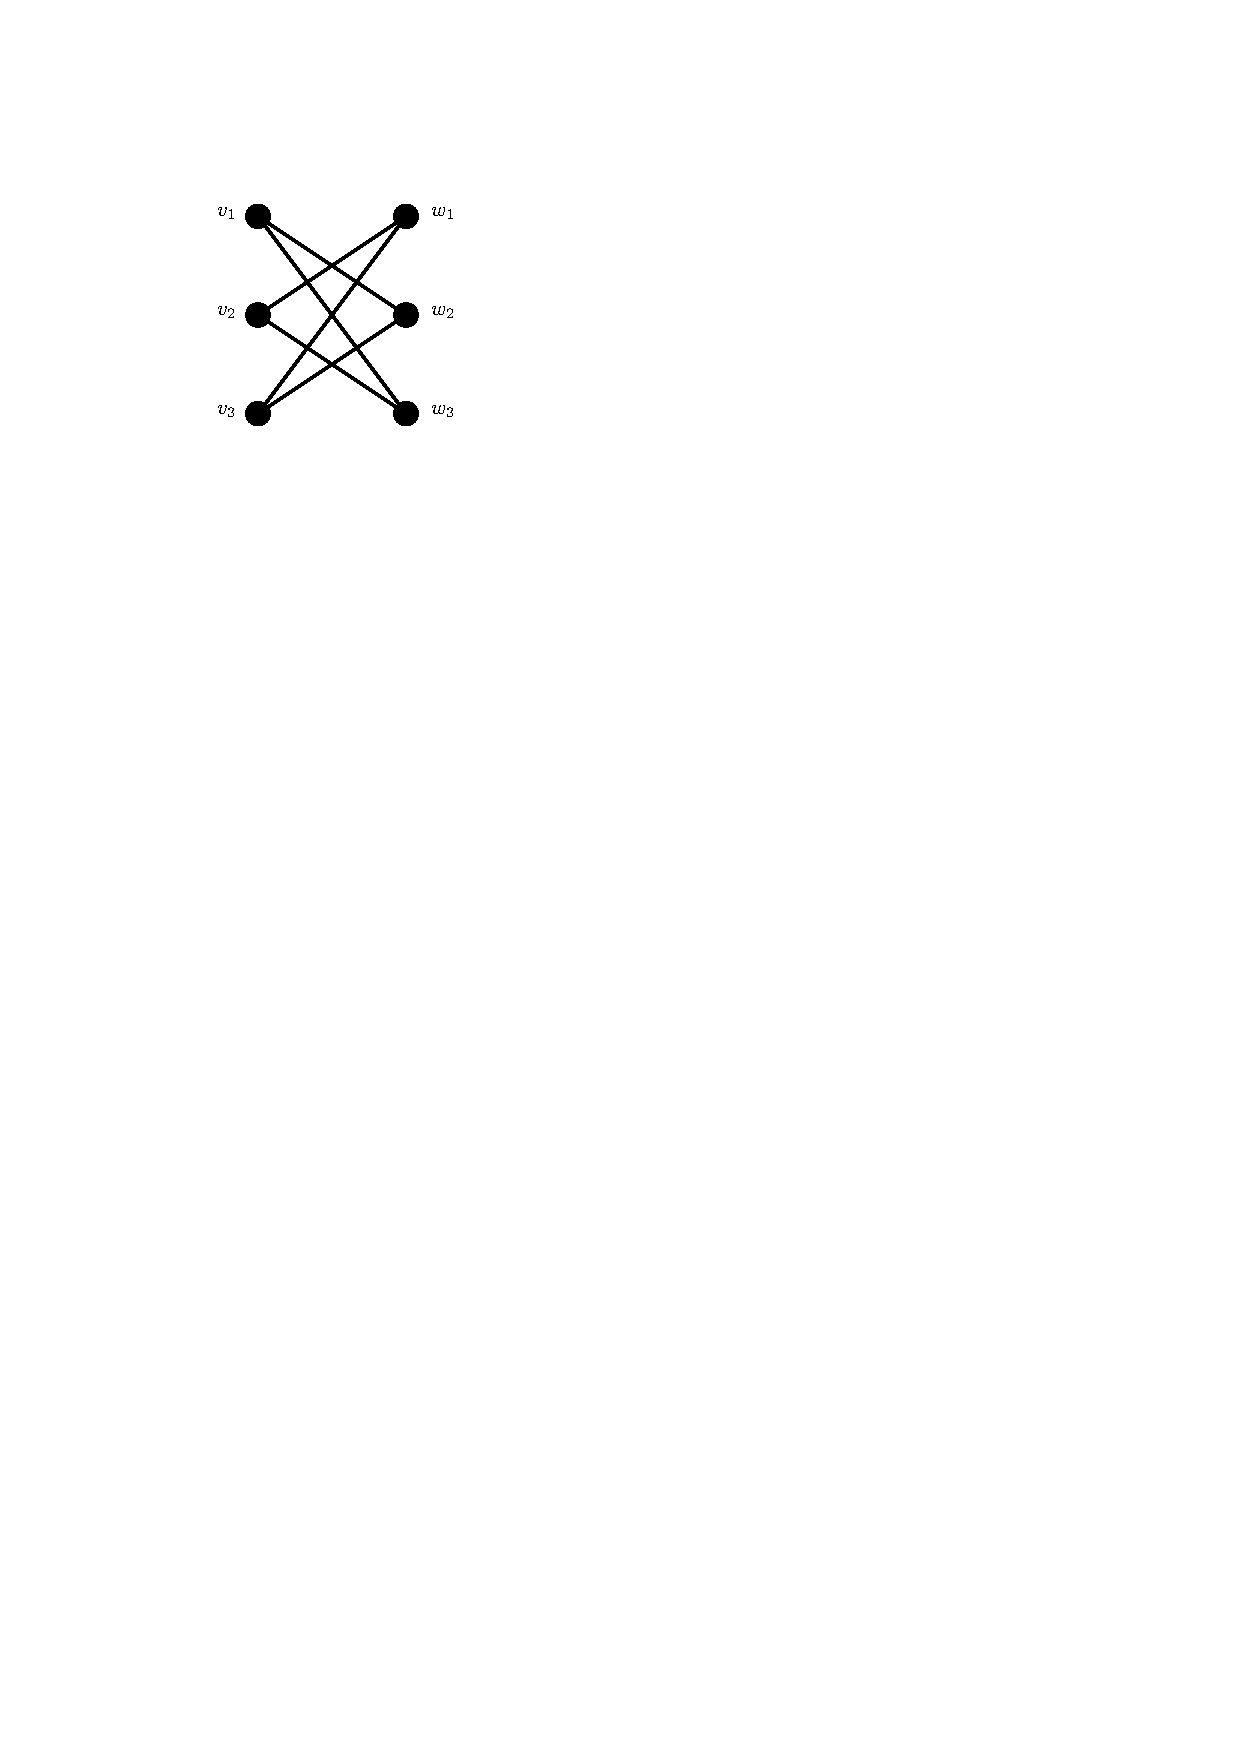
\includegraphics[scale=1.3]{bipartite}
\end{center}


\section*{Problem 1}
A {\bfseries planar graph} is a graph that can be drawn without any edges crossing.
\begin{enumerate}
\item First, show that any subgraph of a planar graph is planar.
\solution{
%The edge set of any subgraph will be a subset of the set of edges in the original planar graph. 
Take any ``planar drawing'' of the original graph---a specific drawing of the planar graph such that no edges in the drawing cross.
From this, we can obtain a drawing of the subgraph, by keeping only the edges in the subgraph. Still no edges cross, so this is a planar drawing of the subgraph.

\emph{Note: do keep in mind that ``planar graph'' is not the same thing as ``planar drawing''.}
}

\item Also, any planar graph has a node of degree at most 5. Now, prove by induction that any graph can be colored in at most 6 colors.
\solution{
We prove by induction. First, let $n$ be the number of nodes in the graph. Then define
\[P(n)=\text{Any planar graph with $n$ nodes is 6-colorable.}\]

\noindent \textit{Base case, $P(1)$:} Every graph with $n = 1$ vertex is 6-colorable. Clearly true since it's actually 1-colorable.

\noindent \textit{Inductive step, $P(n) \rightarrow P(n+1)$:} Take a graph $G$ with $n+1$ nodes. Then take a node $v$ with degree at most 5 (which we know exists because we know any planar graph has a node of degree $\leq 5$), and remove it. We know that the induced subgraph $G'$ formed in this way has $n$ nodes, so by our inductive hypothesis, $G'$ is 6-colorable. But $v$ is adjacent to at most 5 other nodes, which can have at most 5 different colors between them. We then choose $v$ to have an unused color (from the 6 colors), and as we have constructed a 6-coloring for $G$, we are done with the inductive step.

\noindent Because we have shown the base case and the inductive step, we have proved
\[\forall n \in \mathbb{Z}_+:P(n)\]
(Note: $\mathbb{Z}_+$ refers to the set of positive integers.)
}
\end{enumerate}


%\section*{Problem 2}
%A graph $G=(V,E)$ is called \emph{bipartite} if we can divide the vertex set into two parts, the ``left'' part and the ``right'' part, so that every edge has one endpoint in the left part, and one endpoint in the right part.
%The figure below shows an example of a bipartite graph.
%
%For $n$ even, consider a bipartite graph with $n/2$ vertices on the left, labelled $v_1, v_2, \ldots, v_{n/2}$, and $n/2$ vertices on the right, labelled $w_1, w_2, \ldots, w_{n/2}$.
%Put an edge between every node on the left and node on the right, \emph{except} between $v_i$ and $w_i$ for each $1 \leq i \leq n/2$ (the figure shows this graph for $n=6$).
%
%\begin{center}
%    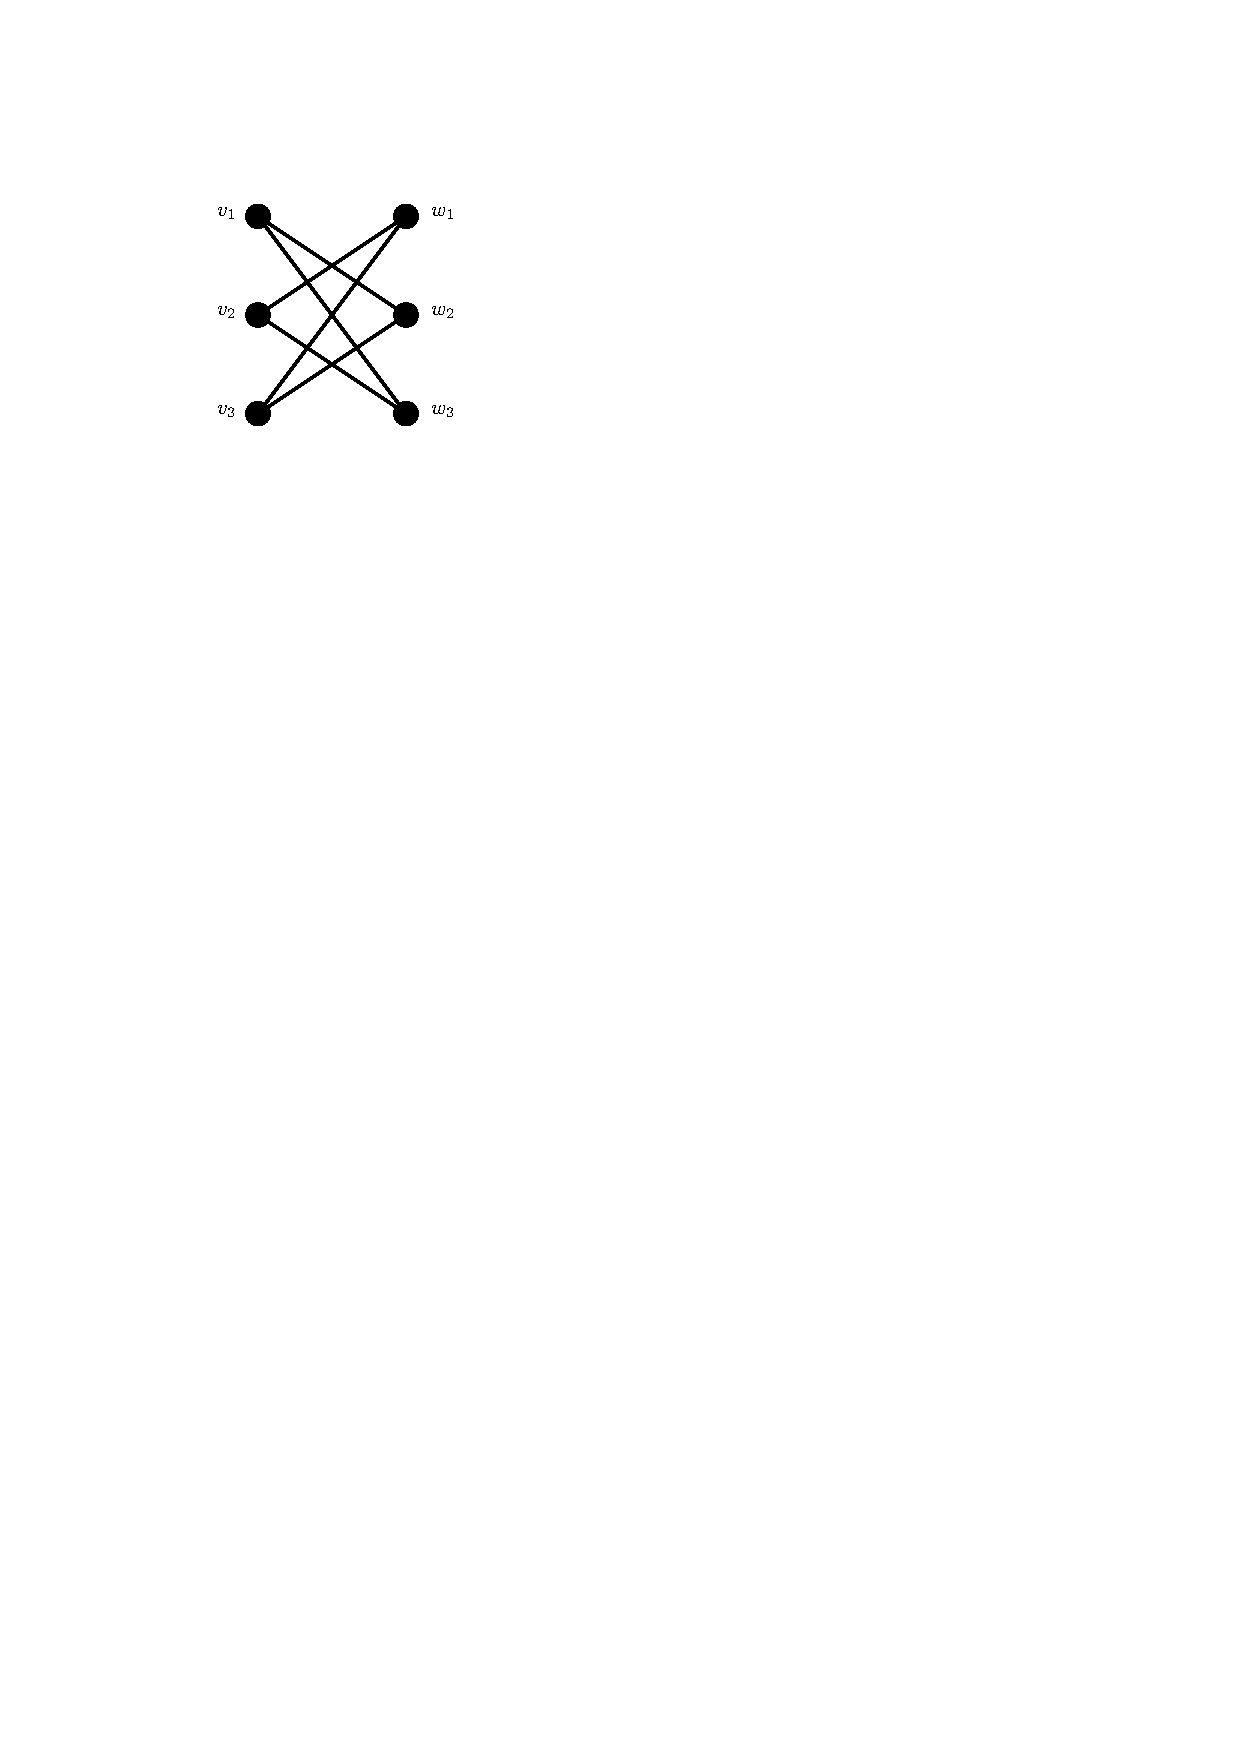
\includegraphics[scale=1.3]{bipartite}
%\end{center}
%\begin{enumerate}[(a)]
%    \item %Show that the basic algorithm uses only 2 colors if the ordering used is 
%        %
%        %\[ v_1, v_2, \ldots, v_{n/2}, w_1, \ldots, w_{n/2}. \]
%        Find an ordering of the vertices where the basic algorithm does well, and uses only $2$ colors.
%    \item Find an ordering where the basic algorithm does \emph{very} badly, and requires $n/2$ colors. 
%\end{enumerate}
%\solution{
%    \begin{enumerate}[(a)]
%        \item        One could take the ordering \[ v_1, v_2, \ldots, v_{n/2}, w_1, w_2, \ldots, w_{n/2}. \]
%            Then each $v_i$ is colored $1$, and each $w_i$ is colored $2$. 
%        \item Take the ordering 
%        \[ v_1, v_2, \ldots, v_{n/2}, w_1, \ldots, w_{n/2}. \]
%        Then $v_1$ and $v_2$ will both be colored $1$. This forces, $v_2$ and $w_2$ to both be colored $2$. Continuing on, we see that $v_i$ and $w_i$ will both be colored with color $i$. This could be proved formally by induction.
%    \end{enumerate}
%}

\section*{Problem 2}
An undirected graph $G$ has \term{width} $w$ if the vertices can be
arranged in a sequence
%
\[
v_1,\ v_2,\ v_3,\ \ldots,\ v_n
\]
%
such that each vertex $v_i$ is joined by an edge to at most $w$
preceding vertices.  (Vertex $v_j$ \textit{precedes} $v_i$ if $j <
i$.)  Use induction to prove that every graph with width at most $w$
is $(w + 1)$-colorable.

(Recall that a graph is \textit{$k$-colorable} iff every vertex can be
assigned one of $k$ colors so that adjacent vertices get different
colors.)


\solution{We use induction on $n$, the number of vertices.  Let $P(n)$
be the proposition that every graph with width $w$ is $(w+1)$
colorable.

\noindent \textit{Base case:} Every graph with $n = 1$ vertex has
width 0 and is $0 + 1 = 1$ colorable.  Therefore, $P(1)$ is true.

\noindent \textit{Inductive step:} Now we assume $P(n)$ in order to
prove $P(n+1)$.  Let $G$ be an $(n+1)$-vertex graph with width $w$.
This means that the vertices can be arranged in a sequence
%
\[
v_1, v_2, v_3, \ldots, v_n, v_{n+1}
\]
%
such that each vertex $v_i$ is connected to at most $w$ preceding
vertices.  Removing vertex $v_{n+1}$ and all incident edges gives a
graph $G'$ with $n$ vertices and width at most $w$.  (If original
sequence is retained, then removing $v_{n+1}$ does not increase the
number of edges from a vertex $v_i$ to a preceding vertex.)  Thus,
$G'$ is $(w+1)$-colorable by the assumption $P(n)$.  Now replace
vertex $v_{n+1}$ and its incident edges.  Since $v_{n+1}$ is joined by
an edge to at most $w$ preceding vertices, we can color $v_{n+1}$
differently from all of these.  Therefore, $P(n+1)$ is true.

The theorem follows by the principle of induction.}

\section*{Problem 3}
A certain Institute of Technology has a lot of student clubs; these
are loosely overseen by the Student Association.  Each eligible club
would like to delegate one of its members to appeal to the Dean for
funding, but the Dean will not allow a student to be the delegate of
more than one club.  Fortunately, the Association VP took Math for
Computer Science and recognizes a matching problem when she sees one.

\begin{enumerate}

\item Explain how to model the delegate selection problem as a
bipartite matching problem.  (This is a \emph{modeling problem}; we
aren't looking for a description of an algorithm to solve the
problem.)

\solution{
Define a bipartite graph with the student clubs as one set of
vertices and everybody who belongs to some club as the other set of
vertices.  Let a club and a student be adjacent exactly when the student
belongs to the club.  Now a matching of clubs to students will give a
proper selection of delegates: every club will have a delegate, and every
delegate will represent exactly one club.}
\end{enumerate}

\section*{Problem 4}

A \term{Latin square} is $n \times n$ array whose entries are the number
$1,\dots,n$.  These entries satisfy two constraints: every row contains
all $n$ integers in some order, and also every column contains all $n$
integers in some order.  Latin squares come up frequently in the design of
scientific experiments for reasons illustrated by a little story in a
footnote\footnote{At Guinness brewery in the eary 1900's, W. S. Gosset (a
chemist) and E.  S. Beavan (a ``maltster'') were trying to improve the
barley used to make the brew.  The brewery used different varieties of
barley according to price and availability, and their agricultural
consultants suggested a different fertilizer mix and best planting month
for each variety.

Somewhat skeptical about paying high prices for customized fertilizer,
Gosset and Beavan planned a season long test of the influence of
fertilizer and planting month on barley yields.  For as many months as
there were varieties of barley, they would plant one sample of each
variety using a different one of the fertilizers.  So every month, they
would have all the barley varieties planted and all the fertilizers
used, which would give them a way to judge the overall quality of that
planting month.  But they also wanted to judge the fertilizers, so they
wanted each fertilizer to be used on each variety during the course of
the season.  Now they had a little mathematical problem, which we can
abstract as follows.

Suppose there are $n$ barley varieties and an equal number of
recommended fertilizers.  Form an $n \times n$ array with a column for
each fertilizer and a row for each planting month.  We want to fill in
the entries of this array with the integers 1,\dots,$n$ numbering the
barley varieties, so that every row contains all $n$ integers in some
order (so every month each variety is planted and each fertilizer is
used), and also every column contains all $n$ integers (so each
fertilizer is used on all the varieties over the course of the growing
season).}

For example, here is a $4 \times 4$ Latin square:
{\Large
\[
\begin{array}{|c|c|c|c|}
\hline
1 & 2 & 3 & 4 \\
\hline
3 & 4 & 2 & 1 \\
\hline
2 & 1 & 4 & 3 \\
\hline
4 & 3 & 1 & 2 \\
\hline
\end{array}
\]
}

\begin{enumerate}

\item

Here are three rows of what could be part of a $5 \times 5$ Latin
square:

{\Large
\[
\begin{array}{|c|c|c|c|c|}
\hline 2 & 4 & 5 & 3 & 1 \\ \hline 4 & 1 & 3 & 2 & 5 \\ \hline 3 & 2 &
1 & 5 & 4 \\ \hline & & & & \\ \hline & & & & \\ \hline
\end{array}
\]
} Fill in the last two rows to extend this ``Latin rectangle'' to a
complete Latin square.

\solution{
Here is one possible solution:

{\Large
\[
\begin{array}{|c|c|c|c|c|}
\hline 2 & 4 & 5 & 3 & 1 \\ \hline 4 & 1 & 3 & 2 & 5 \\ \hline 3 & 2 &
1 & 5 & 4 \\ \hline 1 & 5 & 2 & 4 & 3 \\ \hline 5 & 3 & 4 & 1 & 2
\\ \hline
\end{array}
\]
}
}

%There are some nice connections between Latin squares and graph
%theory.


\item Show that filling in the next row of an $n \times n$ Latin
rectangle is equivalent to finding a matching in some $2n$-vertex
bipartite graph.

\solution{
Construct a bipartite graph as follows. One set of vertices are the
columns of the Latin rectangle, and the other set is the numbers $1$
to $n$. Put an edge between a column and a number if the number has
\emph{not yet appeared} in the column. Thus, a matching in this graph
would associate each column with a distinct number that has not yet
appeared in that column. These numbers would form the next row of the
Latin rectangle.}



%\item The VP's records show that no student is a member of more than
%9 clubs.  The VP also knows that to be eligible for support from the
%Dean's office, a club must have at least 13 members.  That's enough
%for her to guarantee there is a proper delegate selection.  Explain.
%(If only the VP had taken an \emph{Algorithms} class, she could even
%have found a delegate selection without much effort.)
%
%\solution{
%The degree of every club is at least 13, and the degree of every
%student is at most 9, so the graph is
%\emph{degree-constrained}, which implies there
%will be no bottlenecks to prevent a matching.  Hall's Theorem then
%guarantees a matching.}

\end{enumerate}

%%%%%%%%%%%%%%%%%%%%%%%%%%%%%%%%%%%%%%%%%%%%%%%%%%%%%%%%%%%%%%%%%%%%%%%%%%%%%%%

\end{document}
